\chapter{Implementation and Results}
%\section{Implementation}
%explain the test bed platform, block diagram, components, how they are implemented, openserial module implementation, How synchronization is achived between mote. External MAC. packets format of openserial

%Details regarding implementation and/or simulation are given in this chapter. The considered setup and the parameters used are introduced and discussed. Also, the general evaluation methods can be presented. (Note: Code should not be part of this chapter. If it makes sense to introduce it into the thesis, it should be placed in the appendix.)

%\section{Results}
%Results of the performed investigations are presented here. Interpretations for the observed effects are given and the impact of investigations is discussed.

\section{Development and evaluation eastbound interface}
\setcounter{secnumdepth}{3}
Wireless sensor network testbeds allow researchers to conduct experiments, evaluate different channel access algorithms and protocols. In industrial communication latency and reliability play significant role so in our implementation we are concentrating more on these parameters. With wireless testbed it is easy conduct experiments and evaluate different algorithms.

In the process of developing low latency wireless testbed first step is naturally setting up of the low latency network in which latencies can be measured or characterized accurately, The road block for this was openvisualizer. which is necessary for setting of WSN. however OpenWSN was making latency measurement/debugging difficult. So step explored is to figure out a way to set up WSN network without OpenVisualizer, Which involved understanding the type functionalities OpenVisualizer is doing and which functionalities are absolutely necessary.

Through thorough investigation of OpenVisualizer code following functionality found to be implemented.

\begin{enumerate}
	\item Maintaining routing table for nodes in the network for downward traffic using source routing headers.
	\item Communicating motes at the exact super serial RX and TX frame slots.
	\item Controlling/configuring the parameters of sensor network.
	\item Packets read from TUN/TAP interface and then injected to mote via serial after converting to 6LoWPAN format with source routing header.
	\item Lot of Unwanted debug information is sent from stack to OpenVisualizer to make it user-friendly for which at least 2 slots(each slot 15 milliseconds), hence making super frame long and resulting in more latency.
	\item Modules for redirecting packets received from sensor network to wireshark for debugging.
	\item HDLC protocol implementation.
\end{enumerate}

All this data is not sent to host without host asking for it. This is lot of traffic which causes significant latency in overall system.

In the above findings, functionalities which contributed most to latency and made latency characterization is the 5\textsuperscript{th}, Lot of unnecessary debug information was being sent and it was not critical. The next component was TUN/TAP interface which is not needed unless we want want to put the data to internet therefor it was making the OpenVisualizer heavy and complex.

The next step for reducing latency and making measurements easy is to kill OpenVisualizer then PC side tool replacing OpenVisualizer which has minimal functionality necessary for maintaining the network. This PC side tool is developed in Python. In addition to maintaining network, it should ease measurement of latency in different components of system.

OpenVisualizer communicates with openserial driver running in OpenWSN firmware. openserial driver needs to be redeveloped to comply with new functional behavior of Python module(instead of OpenVisualizer) running in the PC. Here new serial packet formats are developed to modularize processing of the control serial packets,data packets, debug packets,error packets.

\subsection{Open serial driver design}
In original implementation data is exchanged over hdlc protocol which further introduces overhead over serial communication. This hdlc protocol overhead is removed to avoid overhead.

Another problem with openserial driver stack information is sent to OpenViusalizer without being asked for, In our design openserial driver sends the necessary data only when it is requested due this only required data at requested time is sent to host. In this design 15ms slots are no longer necessary slot size can also be reduced.


The scheduling of the serial driver is carried out according to super frame timing. openserial driver api's \texttt{openserial\_startOutput},\texttt{openserial\_startInput},\texttt{openserial\_stop} are the function which do all the work.

\texttt{openserial\_startOutput} reads the data queued in output circular buffer transmits this data to host via uart in the SERIALTX slot.

\texttt{openserial\_stop} processes the serial data received from the host in SERIALTX slot, before starting the uart transmission.

\texttt{openserial\_startInput} sends the request frame to host for indicating the SERIALRX slot so that host can send the data.

Above three API's were implemented in OpenWSN originally to schedule the openserial component from MAC layer. In the present design too scheduling is kept same as the original one. Except modification of MAC layer related to serial communication as explained in the last subsection.

Figure

\begin{figure}
	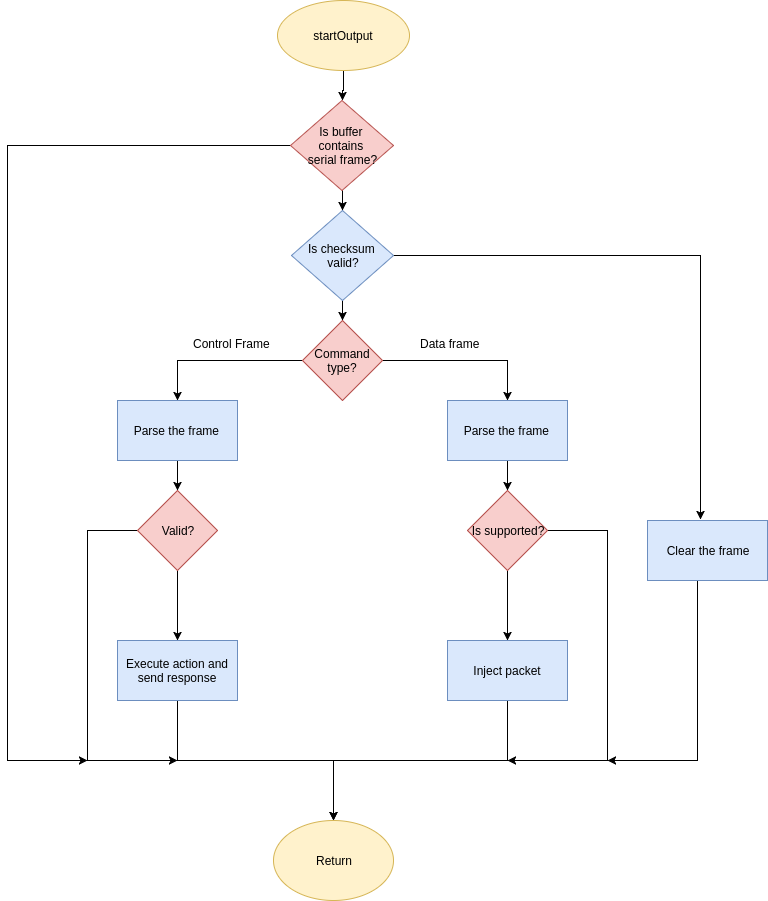
\includegraphics[width=0.7\textwidth,center]{Openserial_startOutput.png}
	\caption{Serial frame processing}
	\label{fig:Openserial_startOutput}
\end{figure}

In the present implementation of openserial driver buffer management and serial data parsing are two main components.
Lets have a look briefly in to the these components.

\textbf{Buffer management}: \newline
Open serial driver manages the data in two circular buffer implementations TX\_BUFFER and RX\_BUFFER of size 256 bytes. When SERIAL\_RX slots are scheduled, hosts send data via uart. Once byte received in the interrupt handlers data is pushed in to SERIAL\_RX buffer. This buffered data is processed in idle slot if any before mote goes in to sleep mode or in SERIAL\_TX slot by calling \texttt{openserial\_stop} at the beginning of SERIAL\_TX slot. 

TX\_BUFFER is used buffering data which needs to sent via serial to host computer. Whenever mote wants send data(Eg:Sending packet received or debug information) It call \texttt{openserial\_printf} This function is part  of open serial driver which buffers this data to TX\_BUFFER. When SERIAL\_TX slot is scheduled this data is popped from TX\_BUFFER and  transmitted via UART. As will be explained later in this chapter, With aim reducing the latency, slot widths in TSCH schedule is reduced as minimal as possible. During this research internship slot width are reduced from 15ms to 6ms, so only a limited amount of data can be sent via serial. One can calculate how much data can sent via particular baudrate with following simple equation.

\begin{equation}
Max\_bytes\_per\_slot = (\frac{baud rate}{10})*slot\_width
\end{equation}

For example at baudrate of 115200 and 6ms slot width, at max 69 bytes can be sent. These numbers have to be kept in mind while sending data via serial. Here while calculating the slot width additional margin of 0.6 ms for USB controller stack and chip processing delay must taken into account.

Sample serial frames(Data frames, command frames)
In the openserial driver to make implementation neat two types of serial frames are implemented, namely data serial frames and command serial frames which are used for network management purpose. For example serial frames which are used for injecting UDP packet data belong to serial data frames category, Serila frames which are used for getting TSCH schedule belong to commnd serial frame category. This type modularization helps to modularize the serial  frame processing logic in openserial driver.

To make serial frames packet processing streamlined, Every serial packet starts with \texttt{0x7e} which indicates beginning of the frame, next byte represents overall length of the packet then comes packet type/subtype and payload.
Lets look at sample serial frames.

Following command frame makes configures the mote as DAGroot. The first byte indicates beginning of the frame, second byte length of the packet excluding \texttt{0x7e} , third byte indicates that it is a control frame, fourth byte represents action of the command i.e to set mote as dagroot.

\begin{table}[H]
	% increase table row spacing, adjust to taste
	\renewcommand{\arraystretch}{1.3}
	\label{meas:set dag root command}
	\centering
	\begin{tabular}{|c|c|c|c|}
		\hline
		\texttt{0x7e} & \texttt{0x03} & \texttt{0x43} & \texttt{0x00} \\
		\hline
	\end{tabular}
	\caption{Serial frame set DAG root}
\end{table}

Following sample command represents command used for injecting UDP packet to network, This frame too follows the same protocol explained above. 3rd byte represents command category as Data related fourth byte represent the specific command types such as UDP injection or TCP injection.

\begin{table}[H]
	% increase table row spacing, adjust to taste
	\renewcommand{\arraystretch}{1.3}
	\label{meas:UDP_inject}
	\centering
	\begin{tabular}{|c|c|c|c||c|c|c|c||c|c|c|c|}
		\hline
		\texttt{0x7e} & \texttt{0x0b} & \texttt{0x44} & \texttt{0x00} & \texttt{0xff} & \texttt{0x02} & \texttt{0x02} & \texttt{0x02} & \texttt{0x02} & \texttt{0x02} & \texttt{0x58} & \texttt{0x01} \\
		\hline
	\end{tabular}
	\caption{Serial frame, Inject UDP packet}
\end{table}

\begin{table}[H]
	% increase table row spacing, adjust to taste
	\renewcommand{\arraystretch}{1.3}
	\label{meas:Explanation}
	\centering
	\begin{tabular}{|c|c|}
		\hline
		\texttt{0x7e} & \texttt{Indicates the beginning of packet} \\
		\hline
  		\texttt{0x0b} & \texttt{Length of the packet excluding 0x7e} \\
  		\hline
  		\texttt{0x44} & \texttt{Indicates the category of packet('D') data packet} \\
  		\hline
  		\texttt{0x00} & \texttt{Subcategory of the packet UDP inject} \\
  		\hline
  		\texttt{ff}\texttt{02}\texttt{02}\texttt{02}\texttt{02}\texttt{02} & \texttt{UDP payload} \\
  		\hline
  		\texttt{5801} & \texttt{Check sum} \\
  		\hline
	\end{tabular}
	\caption{Different fields in a packet}
\end{table}



 The command category that is third byte in very useful for modularizing the processing logic in open serial driver. When processing the packet received, if the open serial driver checks this type, delegates the processing of this packet to respective module(Command processing category or data processing category).

%TODO Explain about, Processing of frames explain if any further information is needed.

\subsection{Network management module}
After open serial driver designed, host side application is needed for handling following functionalities. This a minimal python module implements only the absolutely required functionality. Design idea behind this minimal network management module in contrast to OpenVisualizer is that mote shares the network stats only when this module requests for it(Few exceptions like critical errors and when packet arrived).

\begin{enumerate}
	\item For configuring the network(Setting DAG Root).
    \item Getting network statistics.
	\item Measuring the latency from stack.
	\item Maintaining network topology for downward source routing.
	\item Setting up required TSCH schedule for nodes.
	\item Forms 6LoWPAN packet from industrial control system data.
	\item Handles serial communication.
\end{enumerate}

Lets go into details of the each functionality, briefly look at the purpose they serve.

When all the nodes are running for the network to start functioning at least one node has to DAG root it acts like a central collection node. DODAG is formed according to APL protocol by keeping this node are root node. Network forming starts from here, i.e as soon as this node is made root node this transmits the advertisement packets about presence of the network other nodes join this network. therefore one node has to be dagroot the functionality is achieved by sending a serial command frame.

Getting network statistics is very important for debugging and to get information about network such as schedule,neighbors etc, This functionality is again implemented based command response basis only, When a host wants to know stack information corresponding command is sent, network statistics is returned in the response frame.

Latency plays a very significant role in industrial communication, Measuring latency is required, it may be latency due to communication stack,MAC schedule or serial etc. To make these measurements easy, Few options are provided in the framework where stack injects the data, latency info is taken from stack sent through response frame this information is saved in json format for further processing.
 
In OpenWSN stack upward routing is implemented RPL\cite{GADDOUR20123163} which based on DOADG's. RPL works for upward routing and it is specifically designed for data collection networks. OpenWSN uses achieves downward routing using source routing mechanism, the which needs to routed contains the route, Each node in the path looks at the packet forwards according to route specified. DAG root runs only the MAC layer in OpenWSN stack. When packet needs to sent downward from DAG root, that packet should contain routing information for this DAGroot must be aware of the complete network, This is achieved in OpenWSN with DAO messages. All the nodes of network send information about their parents to DAGroot, this information is relayed to host application where routing table is built before injecting packet to DAGroot host side application creates source routing header. This was in OpenVisualizer too, Same implementation is adapted to Network management module.

Handling schedule is one more feature required for adjusting the schedule according to traffic/latency requirements. Because of this reason three specific commands are implemented view schedule,add/remove RX or TX slots.

In host computer industrial control system(Either sensor/controller) is running it sends calculated/sensed data via sockets this data needs to be received,converted to 6LoWPAN packet. This functionality too is implemented as as part of this python module.

Finally serial communication functionality is implemented through multiple threads avoid latency in the host application. Serial communication is handled by separate threads with necessary synchronization between the two.

\begin{figure}[H]
	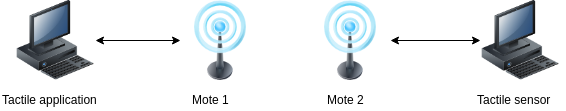
\includegraphics[width=0.8\textwidth,center]{Control_loop_setup_1.png}
	\caption{Experimental setup}
	\label{fig:experimental_setup_loop1}
\end{figure}

\section{LLDN schedule construction}
To achieve low latency as MAC layer is modified, 802.15.4e MAC mechanism allows synchronization with ack's too. However this synchronization based on ack's make slot width long. In turn increases latency. To avoid this ack's are removed from the schedule and synchronization for of network nodes is done only through beacon frame's with their frequency increased. Sample schedule is shown below. \cite{Yagiz}

In the schedule TXRX frame is used for sending beacon frames hence allowing all  nodes in the network(star topology) to synchronize with their parents, in this case with dagroot.

Typical schedule in the present implementation.

\begin{figure}[H]
	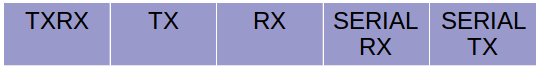
\includegraphics[width=0.6\textwidth,center]{schedule_table.png}
	\caption{schedule}
	\label{fig:schedule}
\end{figure}

\section{Modified OpenWSN External MAC}
External MAC is a mechanism to choose when data has to be sent from user application running in host computer to mote and vice versa. Since the mote has single micro controller this communication time also should be part of super frame schedule. In order to do that serial communication timing is accommodated in schedule through serial RX and TX slots, These slots are used  for communicating with host computer running user application. The mechanism is as explained below. In the schedule as soon serial RX starts MAC layer calls the start input function of the openserial driver, then a request frame is sent to host to indicate that it is ready to receive. Once the host receives request frame it sends the data to mote. In the original OpenWSN implementation request frames were sent once in every super frame. In this design user application cannot inject multiple data packets in one superframe although enough slots are available.  This is not well suited for achieving low latency communication. In our design the MAC layer is modified in such a way that for every SERIALRX slot request frame is sent to host. In this design modification data can be sent from host computer in every SERIALRX slot.

%explain all the work done during the setup, Understanding the OpenWSN stack, problems with openvisualizer not designed for achieving low latency, Difficult to characterize the delay components, Lot unnecessary data is shared to OpenVisualizer to make user friendly which makes systematic measurement/latency characterization of the different components hard. For example lot of data is sent via serial port hence more delay is attributed to serial communication. Formulating the optimal schedule with minimal slots for achieving low latency. Characterization of MAC layer delay components, measurement of delay due to spi interface to make slot as small possible to allow only the maximum packet transmission time. Explain the design openserial driver modular design for collecting the stack information and for the management of network, such as getting the schedule adding different types of slot(RX,TX),removing the acknowledgement to improve latency,Doing synchronization with the beacon packet(And their frequency is increased to avoid the desynchronization).
%
%Explain the minimal set of commands implemented in openserial driver presently.
%
%Explain the development of python mudules in the PC side which communicates with mote via serial communication for management of the network, Network information to maintain the routing table for source routing,data packet receiving sending to PC side control application via UDP sockets,Data packet injection received from the Control application via UDP sockets.

\section{Eastbound delay characterization}
This document describes the characterization of delays involved in the eastbound interface of wireless sensor network setup. For the characterization of delays open source IoT stack OpenWSN is considered.

\subsection{Setup}
In the experimental setup Zolertia-Z1 mote running OpenWSN is considered.
Mote is connected to host running user application via serial interface.
The packets generated in the application are injected into the mote through serial interface.
For Z1 mote serial communication is done over a USB to serial converter module.
This serial interface involves USB to UART converter from Silicon Laboratories(CP2102).
This chip converts the serial data to usb packets(conversion introduces the delay).

USB is not a ideal communication protocol for achieving real time communication especially if the slave device is bulk type device.
USB controller schedules the bus access to the bulk devices based bus availability and latency is not guaranteed. This latency varies depending on how many devices connected to the USB controller and also on the type of end points they have.
For example: If more devices with interrupt and isochronous end points are connected then bulk devices will be deprived from the bus access, since those(interrupt and isochronous) end points have higher priority than bulk end points.
When the mote sends data to host there is one more additional delay involved called USBtimeout value of chip. This delay caused because cp2012 chip waits for the next byte for (18/baudrate) duration before forming a USB packet and transmitting it. In the current design host sends data to mote only after receiving a request frame.When SERIALRX slot starts, mote sends request frame. Due to USBtimeout duration request frame is delayed by USBtimeout duration.
This delay affects the overall latency of the system.
\begin{figure}[!h]
	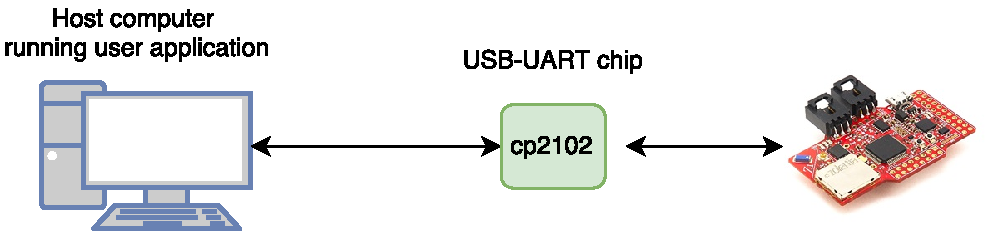
\includegraphics[width=0.5\textwidth,center]{setup.pdf}
	\caption{experimental setup.}
	\label{fig:setup}
\end{figure}

\subsection{Evaluation}
Latency in the eastbound interface has a contribution mainly from four components, Processing and USB polling delay at host($T_{host}$), USB transmission and protocol overhead delay($T_{usb}$), UART transmission delay($T_{serial}$) and USB-UART chip processing delay($T_{chip}$) so total delay is sum these delay components as represented by the following equation.

\begin{equation}
T_{total} = T_{host} + T_{chip} + T_{usb} + T_{serial}
\end{equation}

The $T_{host}$ specific delay is due to USB driver and USB controller. In the experimental set up this value is found to vary as plotted in ~\ref{fig:Chip_ack_delay} on page ~\pageref{fig:Chip_ack_delay}.

%TODO update the explanation with correct numbers.

The protocol overhead delay is due to inherent nature of USB protocol.
This delay comprises of the time involved in sending IN,OUT,ACK packets plus data transmission time.
Once the data from host is received at the USB to serial converter chip. This data is transmitted to mote through serial communication. This delay is highest among all delays and it directly depends on the baud rate used.
In the experimental setup 115200 baud rate is used, which results in 86.6 microseconds delay for transmitting a single byte.

Following figure shows the plot total eastbound delay versus data size, The delay is almost linear function of data size. This dependency is driven mainly by $T_{serial}$

\begin{figure}[H]
	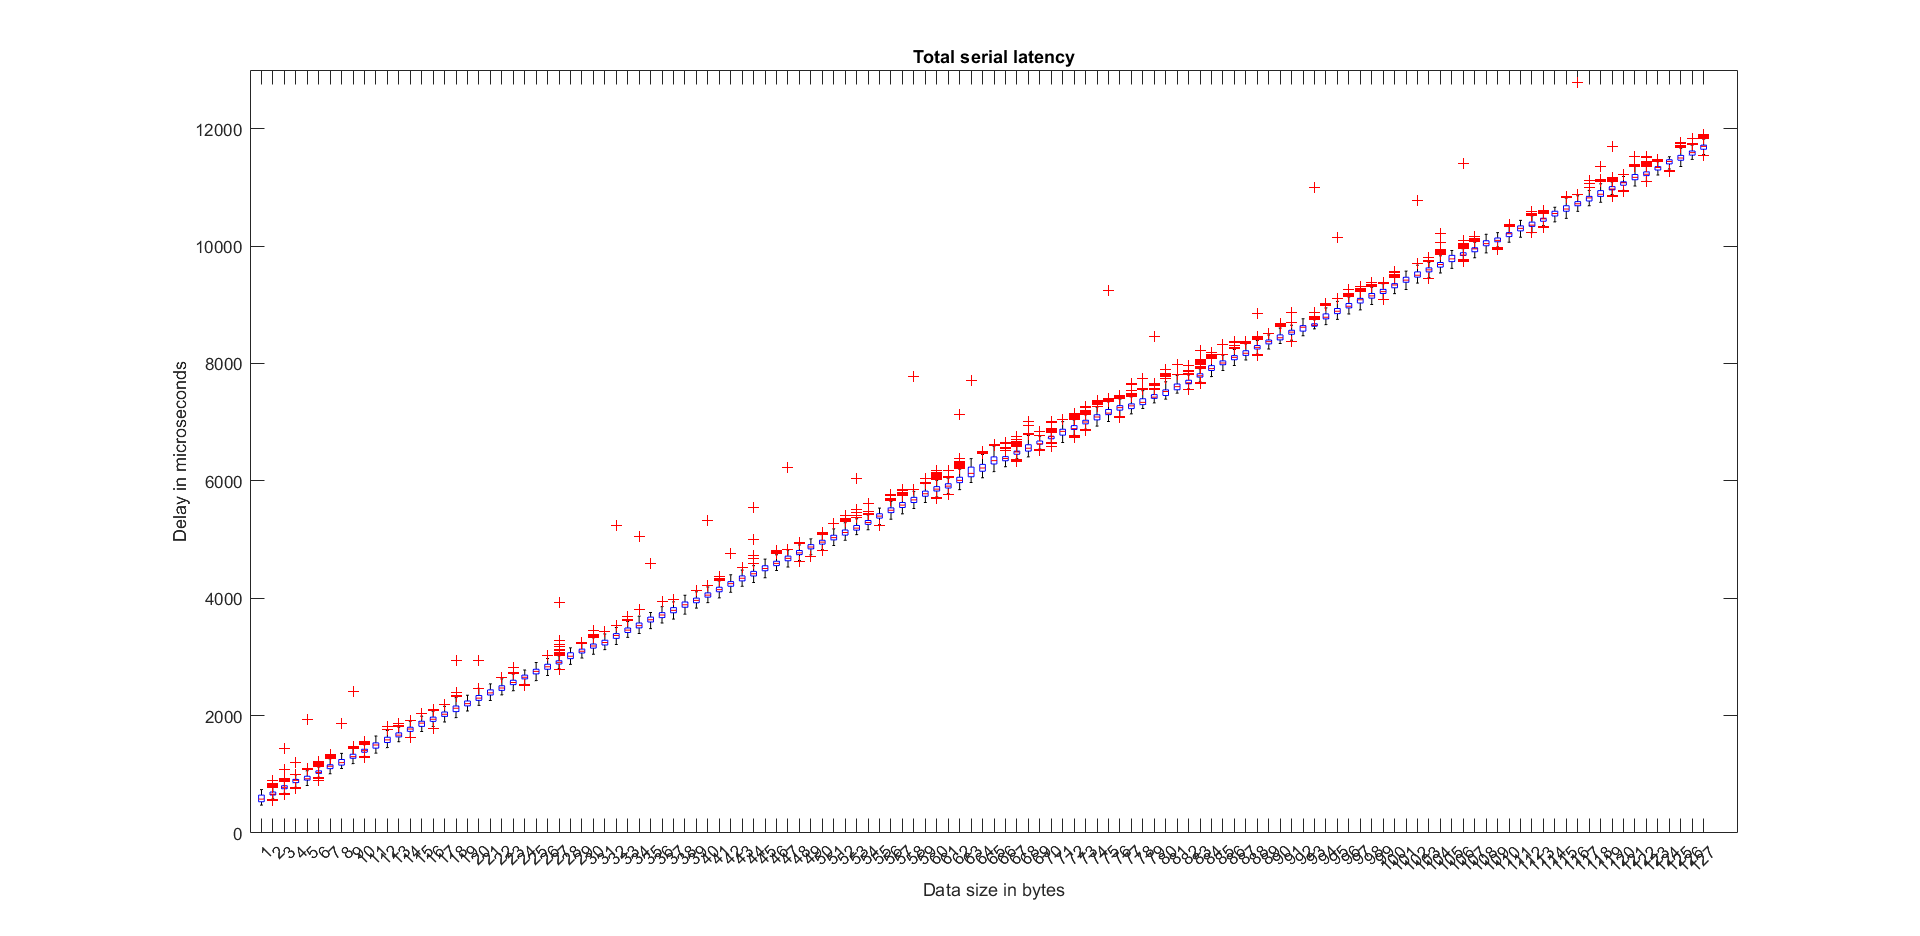
\includegraphics[width=1\textwidth,center]{untitled3.png}
	\caption{Total serial latency}
	\label{fig:Total_serial_latency}
\end{figure}


At last, chip delay. this delay is measured by taking USBmon logs to identify how much delay chip is taking for sending ack's after receiving the USB packet. This delay also found to be significant. Please see the plot ~\ref{fig:Host_polling_and_stack_delay} on page ~\pageref{fig:Host_polling_and_stack_delay}.


For the evaluation of latency, four delay contributors should be considered separately. $T_{host}$ host specific delay is obtained by subtracting chip ack delay, UART delay and USB overhead, it is obtained from measurements.
It can varies from based on the packet%TODO add exact numbers after looking at the graphs.


\subsubsection{Chip ack processing delay}
This delay is the time taken from CP2102 USB-UART chip to send the USB ack after USB packet is sent, With the measurements from USBmon it is found to very significant. This values found to be not constant instead stochastic except USB timeout value.

As discussed earlier cp2102 chip has a parameter called USBtimeout. This is the time after which cp2102 chip starts sending received uart bytes as usb packets, This value is dependent on the baud rate.
At 115200 baud rate USBtimeout value is 156 $\mu$s. This delay is required when data is sent from mote to host, Since waits for 156 $\mu$s before sending data to host. This value is constant hence not included in chip ack delay plot.

Chip ack processing delay is data size dependent with data size this value increase with significant increase when packet bigger than 64 bytes. This increase is because chip has to wait for another USB data packet before sending the ack to host. Chip ack delay values are plotted in figure ~\ref{fig:Chip_ack_delay} on page ~\pageref{fig:Chip_ack_delay}.


\begin{figure}[H]
	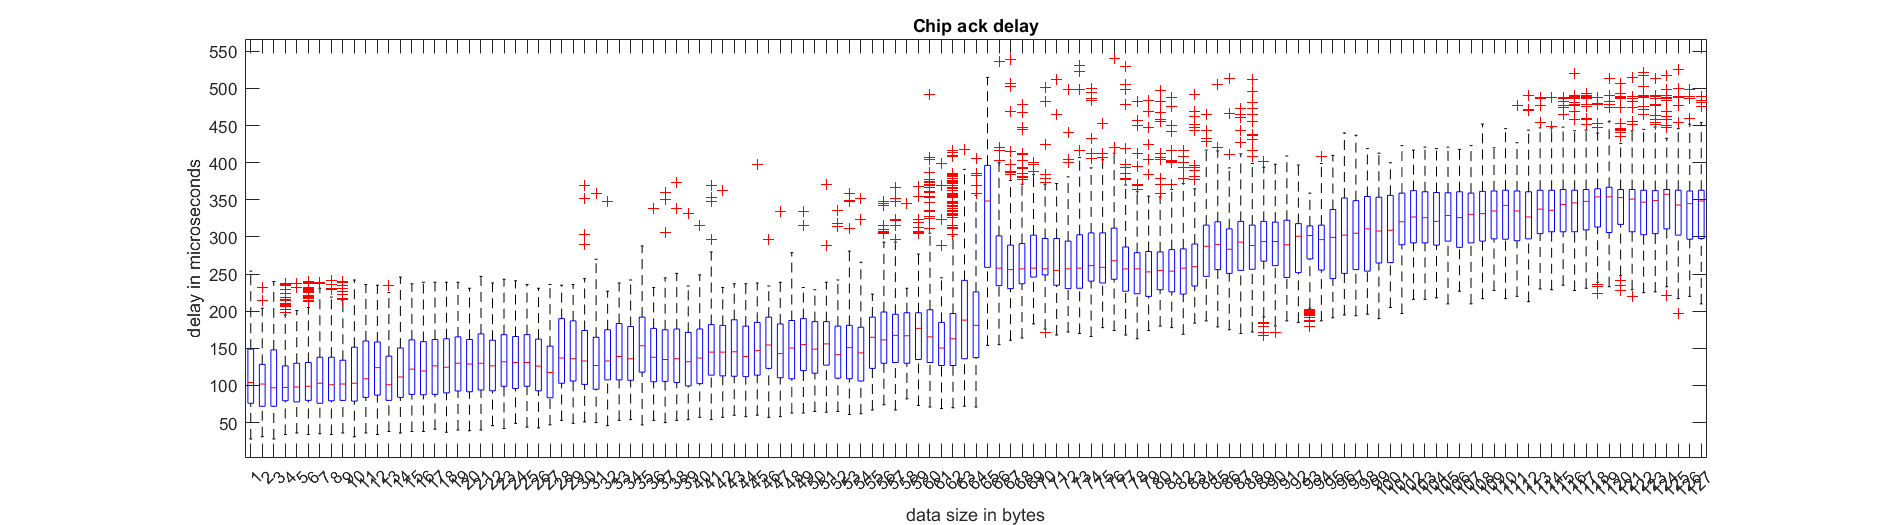
\includegraphics[width=1.4\textwidth,center]{untitled.png}
	\caption{Chip ack delay}
	\label{fig:Chip_ack_delay}
\end{figure}

\subsubsection{USB transmission and protocol overhead delay($T_{usb}$)}
The next delay component is USB communication delay. This delay is calculated by taking into account speed of USB port and protocol overheads involved.
In the present experimental setup cp2102 chip supports USB full speed, hence the throughput of USB is 12 Mbps.
The cp2102 chip has bulk in and out end points with maximum packet size of 64 bytes, that means data is transported in 64 byte USB packets.
We have used python pyserial module to read received data.
USB protocol is host initiated bus, Data is sent from the slave device only when host requests data.
In our experimental setup host sends IN token(size 5 bytes) when serial.read() is called.
Host application is continuously sending the serial read in infinite while loop.
When device has data, it sends data to host.
After receiving request frame host application sends USB data packets to the device in 64 byte packets.
One USB read transaction is represented in the following figure.\cite{Craig.Peacock@beyondlogic.org}

\begin{figure}[h]
	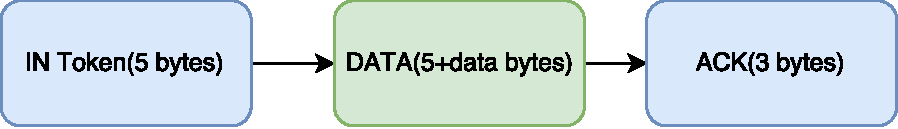
\includegraphics[width=0.5\textwidth,center]{read_trans.pdf}
	\caption{read transaction from USB slave device.}
	\label{fig:read_trans}
\end{figure}

Three USB packets are exchanged for receiving request frame.
IN token,DATA,ACK packet with size 3,5+data bytes length and 3 bytes respectively with two inter packet delay of 3 bytes wide(2 $\mu$s). 
Total time is 12 $\mu$s can be attributed to USB protocol overhead. As we will in the next section this part has very compared serial interface. In this delay USB stack and USB controller delay have huge components.

User application running in host injects data into mote.  One USB write transaction is represented in the following figure.

\begin{figure}[h]
	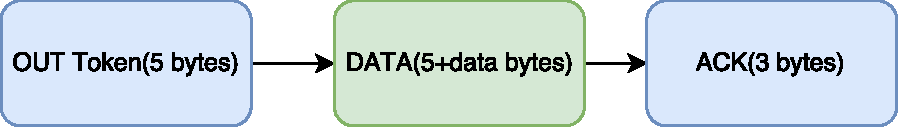
\includegraphics[width=0.5\textwidth,center]{out_trans.pdf}
	\caption{write transaction to USB slave device.}
	\label{fig:write_trans}
\end{figure}

In the experimental setup packet with 12 bytes of user data is considered, including the lowpan headers,source routing header and control bytes of openserial module total packet size becomes 54 bytes. Three packets are exchanged in write transaction with packet size 5,(5+54) and 3 bytes respectively with two inter packet delay of 3 bytes results in 49 $\mu$s.

In the above plot, It is observable that there is constant delay, Above which delay increases weakly until 64 bytes this is reasonable as stack needs make operations with data.

From the plot it is evident that $T_{usb}$ reduces drastically when packet size is more than 64 bytes. This reduction is because, For bulk devices USB controllers try to achieve high throughput by forming packets of maximum packet if possible, To do this USB controller waits for fixed time. We didn't find any value in the data sheet  however from measurements(Combined delay of stack and timeout value) it approximately 180 microseconds.

\begin{figure}[H]
	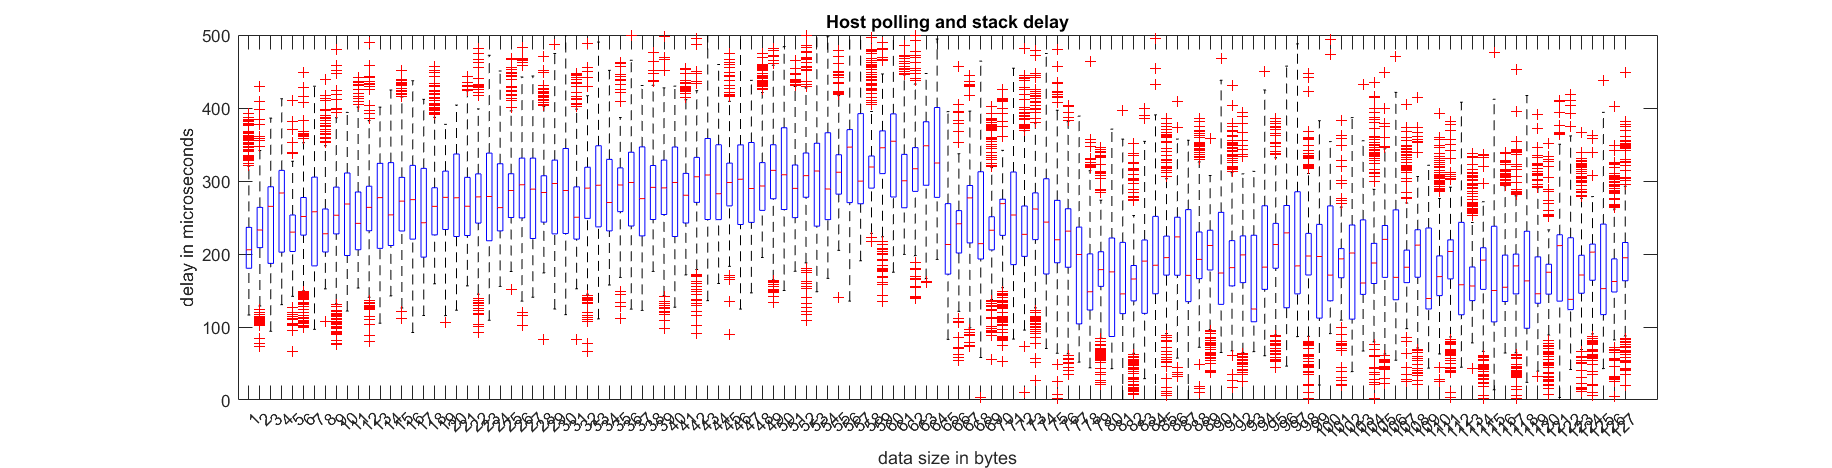
\includegraphics[width=1.4\textwidth,center]{untitled2.png}
	\caption{Host polling and stack delay}
	\label{fig:Host_polling_and_stack_delay}
\end{figure}

\subsubsection{UART transmission delay($T_{serial}$)}
Lets look at the delay due to uart transmission time and receiving time.
This delay is the major contributor to the latency of system, since this value is highest among all the delays. varies linearly with the packet size.
For transmitting one byte at 115200 baud rate 86.6 $\mu$s is needed.

Following plot shows variation of uart delay versus number of uart bytes.
\begin{figure}[H]
	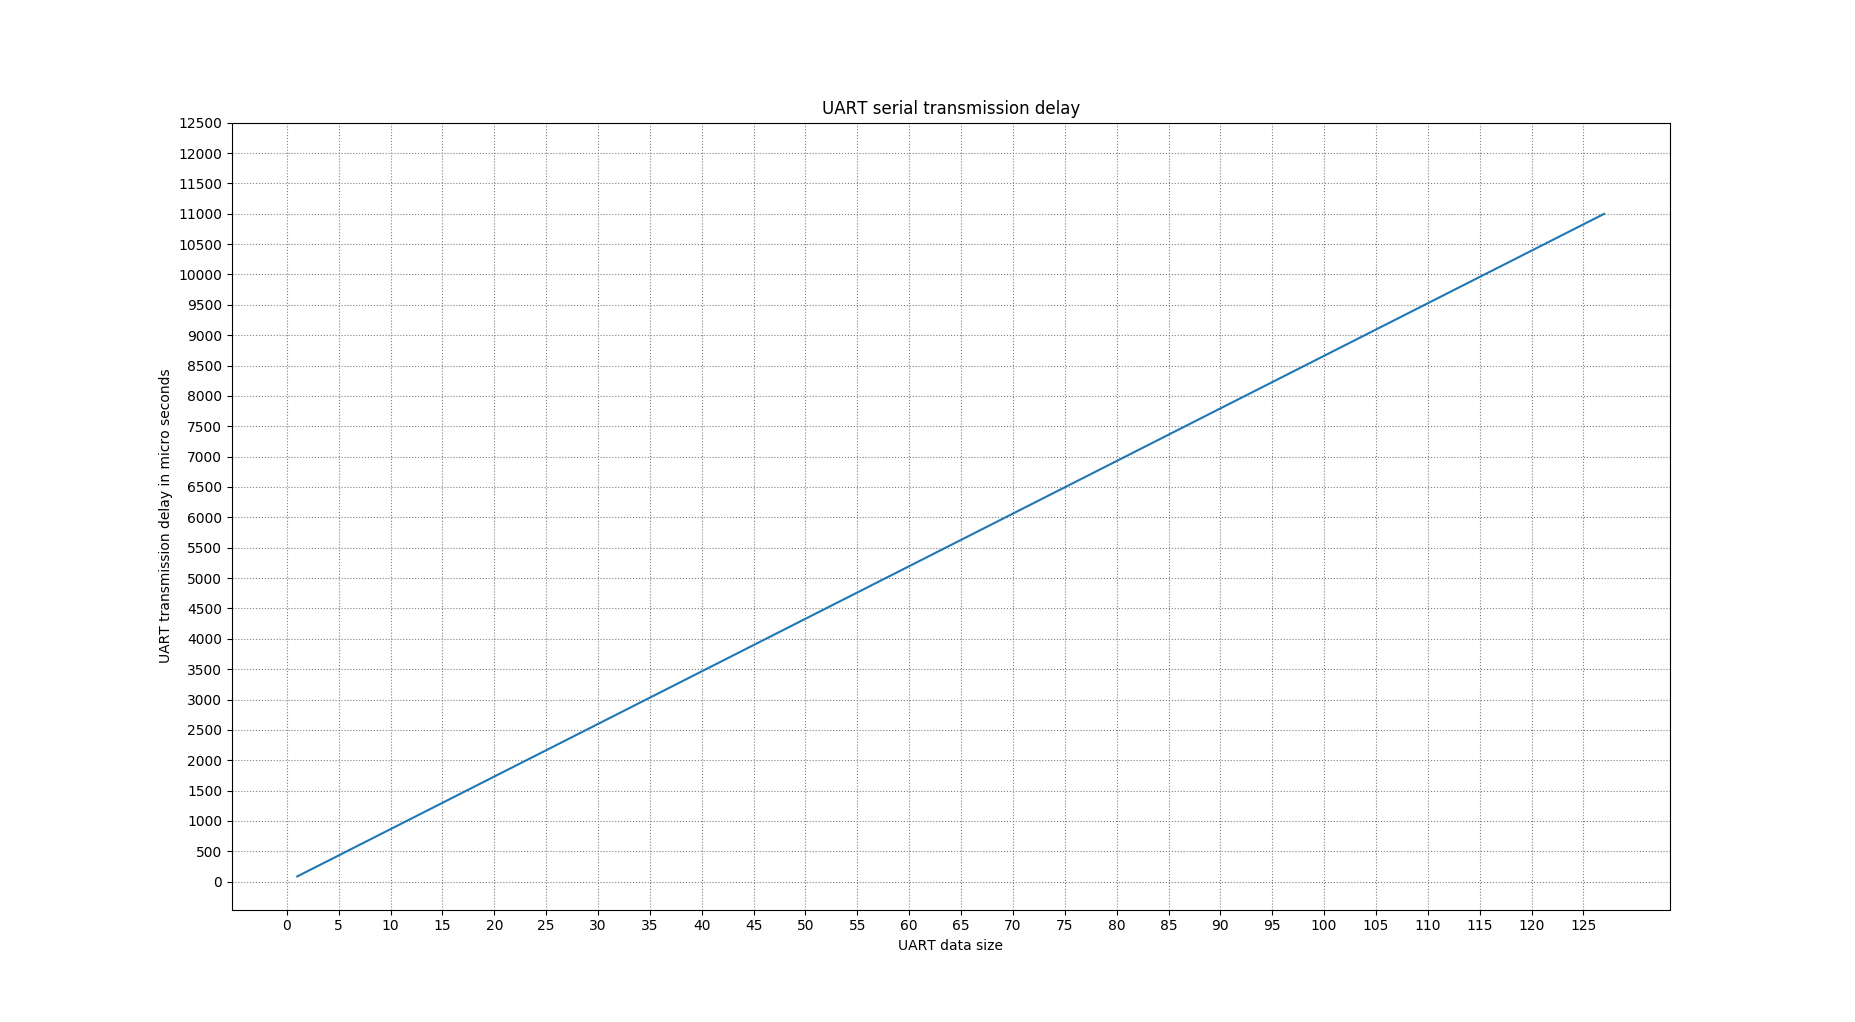
\includegraphics[width=1\textwidth,center]{UART_tx_delay.png}
	\caption{UART TX/RX delay}
	\label{fig:UART transmission delay}
\end{figure}

If we compare above plot with ~\ref{fig:Total_serial_latency} UART tx delay's linear dependency can be clearly seen. So it can be concluded that with bounded offset's of $T_{host}$  and $T_{chip}$ serial latency is a linear function of packet size.

Total delay from east bound interface for data packet is sum of USB stack and controller delay specific  delay($T_{host}$), USB transmission and protocol overhead($T_{usb}$),USB-UART chip processing delay($T_{chip}$) and UART transmission delay($T_{serial}$).
%\begin{table}[H]
%	% increase table row spacing, adjust to taste
%	\renewcommand{\arraystretch}{1.3}
%	\caption{Measurements with Z1 for 54 byte serial data}
%	\label{meas:eastbound1}
%	\centering
%	\begin{tabular}{|c|c|c|}
%		\hline
%		& estimated ($\mu$s)& measured ($\mu$s) \\
%		\hline
%		Z1 & 2851 & 2880 \\
%		\hline
%	\end{tabular}
%\end{table}

Similar estimation and measurement is carried out for a serial packet of length 90 bytes.
Only difference in estimation from previous calculation is that data needs to be sent in two USB packets in chunks of 5(header) + 59(data) and 5(header)+31(data) bytes so extra 5 byte header of second packet and 3 byte interpacket delay needs to taken into account. Results are shown in the following table.

%\begin{table}[H]
%	% increase table row spacing, adjust to taste
%	\renewcommand{\arraystretch}{1.3}
%	\caption{Measurements with Z1 for 90 byte serial data}
%	\label{meas:eastbound2}
%	\centering
%	\begin{tabular}{|c|c|c|}
%		\hline
%		& estimated ($\mu$s)& measured ($\mu$s) \\
%		\hline
%		Z1 & 4464 & 4500 \\
%		\hline
%	\end{tabular}
%\end{table}

\section{Communication stack processing delay}
Communication stack  processing delay is due the processing of data packet in OpenWSN stack before it is stored in a queue. This processing involves adding UDP headers, Compressing UDP headers, Adding checksum,IPv6 headers for routing,Converting packet to 6LoWPAN from IPv6,Including MAC headers at the sixtop layer, then packet is pushed in to queue which is later read by MAC layer and transmitted.

In out experiment setup delay is measured from openserial driver where UDP packet is injected until it queued in transmission buffer. This delay found to be weakly dependent on packet size.

Following figure shows plot of stack processing delay versus UDP payload size. Y-axis represents number of ticks taken for a particular data size(each tick corresponds to 30 microseconds).

\begin{figure}[H]
	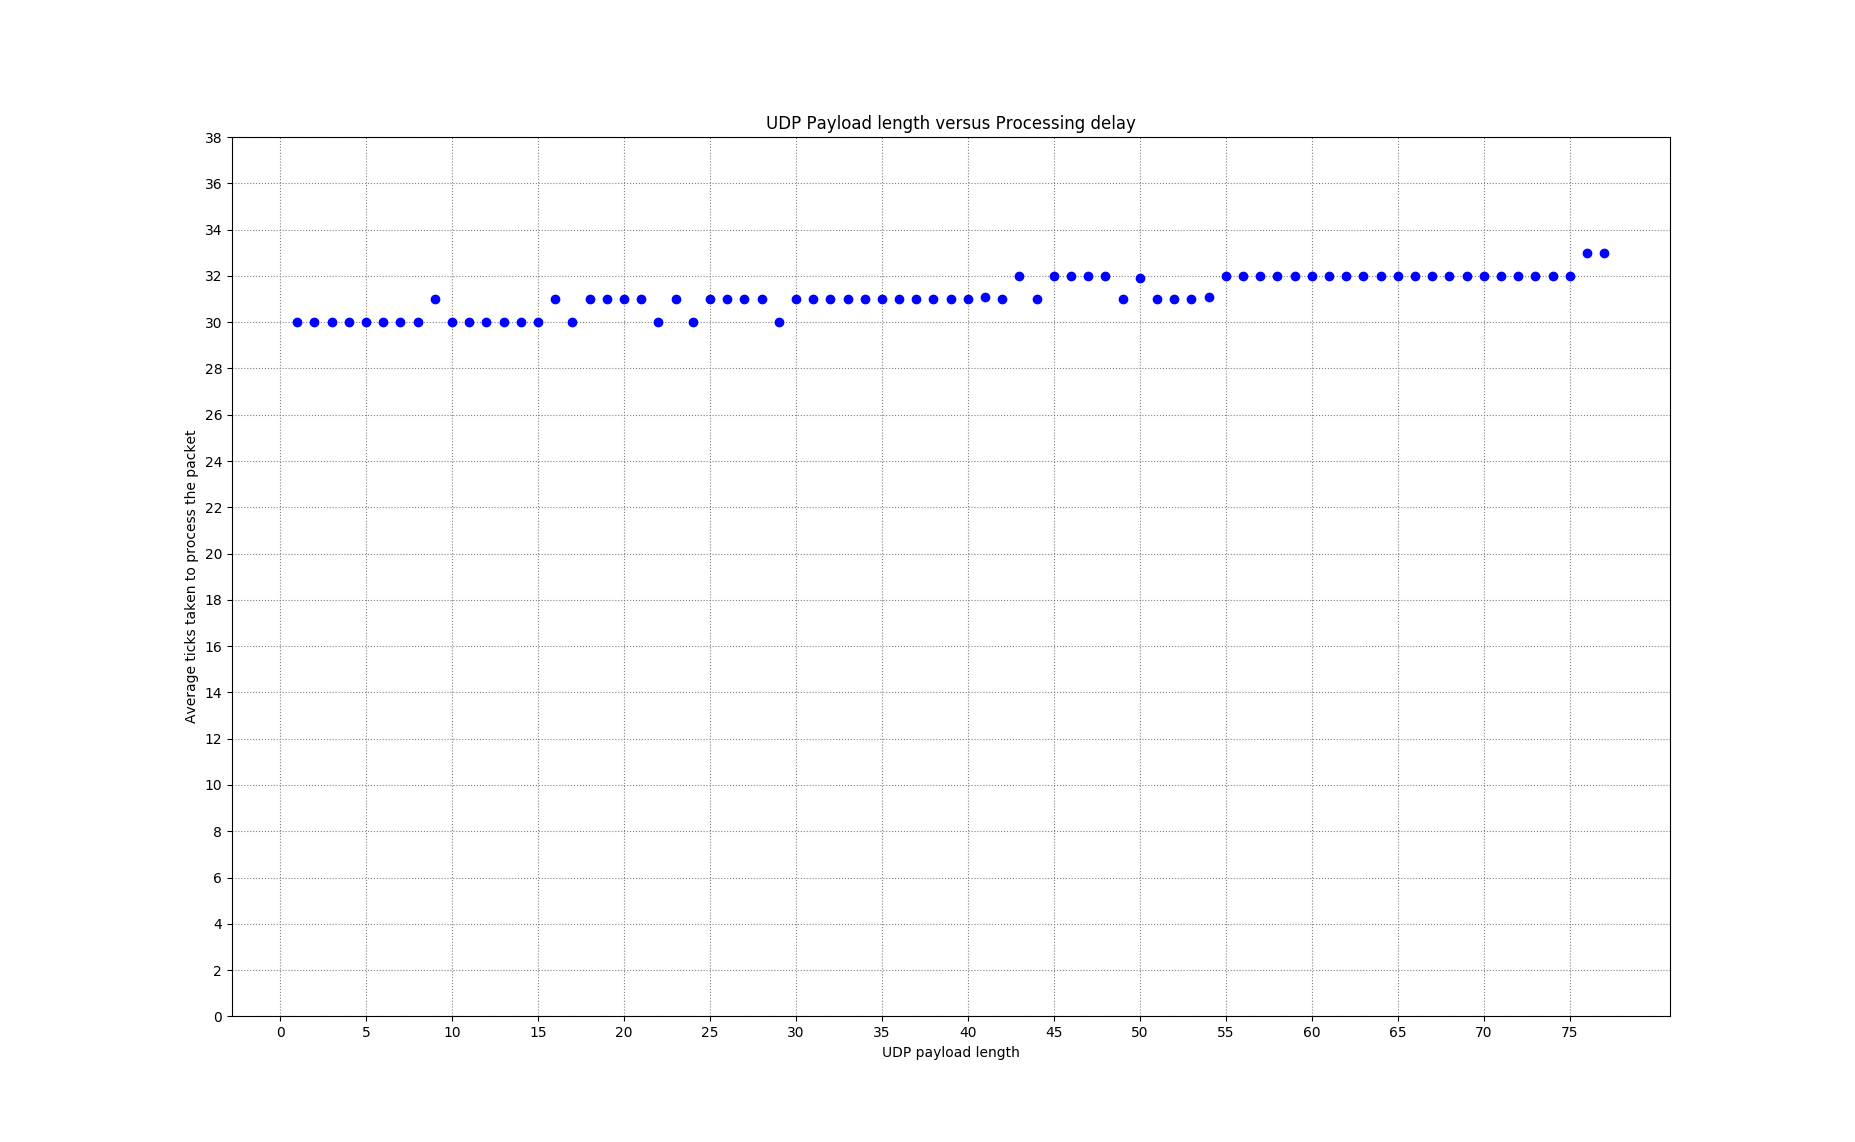
\includegraphics[width=0.8\textwidth,center]{UDP_Packet_processing_delay.png}
	\caption{UDP packet processing delay.}
	\label{fig:write_trans}
\end{figure}
